\documentclass[11pt,compress,t,notes=noshow, xcolor=table]{beamer}
\usepackage[]{graphicx}\usepackage[]{color}
% maxwidth is the original width if it is less than linewidth
% otherwise use linewidth (to make sure the graphics do not exceed the margin)
\makeatletter
\def\maxwidth{ %
  \ifdim\Gin@nat@width>\linewidth
    \linewidth
  \else
    \Gin@nat@width
  \fi
}
\makeatother

\newcommand{\citebutton}[2]{%
\beamergotobutton{\href{#2}{#1}}%
}

\newcommand{\blu}[1]{\textcolor{blue}{#1}}
\newcommand{\org}[1]{\textcolor{orange}{#1}}
\newcommand{\ques}{\textbf{\textcolor{red}{Question:  }}}
\newcommand{\questionssofar}{\begin{frame}\frametitle{Any questions?}\end{frame}}

\newcommand\warning{%
 \makebox[1.4em][c]{%
 \makebox[0pt][c]{\raisebox{.1em}{\scriptsize!}}%
 \makebox[0pt][c]{\color{red}\normalsize$\bigtriangleup$}}}%

\definecolor{fgcolor}{rgb}{0.345, 0.345, 0.345}
\newcommand{\hlnum}[1]{\textcolor[rgb]{0.686,0.059,0.569}{#1}}%
\newcommand{\hlstr}[1]{\textcolor[rgb]{0.192,0.494,0.8}{#1}}%
\newcommand{\hlcom}[1]{\textcolor[rgb]{0.678,0.584,0.686}{\textit{#1}}}%
\newcommand{\hlopt}[1]{\textcolor[rgb]{0,0,0}{#1}}%
\newcommand{\hlstd}[1]{\textcolor[rgb]{0.345,0.345,0.345}{#1}}%
\newcommand{\hlkwa}[1]{\textcolor[rgb]{0.161,0.373,0.58}{\textbf{#1}}}%
\newcommand{\hlkwb}[1]{\textcolor[rgb]{0.69,0.353,0.396}{#1}}%
\newcommand{\hlkwc}[1]{\textcolor[rgb]{0.333,0.667,0.333}{#1}}%
\newcommand{\hlkwd}[1]{\textcolor[rgb]{0.737,0.353,0.396}{\textbf{#1}}}%
\let\hlipl\hlkwb

\usepackage{framed}
\makeatletter
\newenvironment{kframe}{%
 \def\at@end@of@kframe{}%
 \ifinner\ifhmode%
  \def\at@end@of@kframe{\end{minipage}}%
  \begin{minipage}{\columnwidth}%
 \fi\fi%
 \def\FrameCommand##1{\hskip\@totalleftmargin \hskip-\fboxsep
 \colorbox{shadecolor}{##1}\hskip-\fboxsep
     % There is no \\@totalrightmargin, so:
     \hskip-\linewidth \hskip-\@totalleftmargin \hskip\columnwidth}%
 \MakeFramed {\advance\hsize-\width
   \@totalleftmargin\z@ \linewidth\hsize
   \@setminipage}}%
 {\par\unskip\endMakeFramed%
 \at@end@of@kframe}
\makeatother

\definecolor{shadecolor}{rgb}{.97, .97, .97}
\definecolor{messagecolor}{rgb}{0, 0, 0}
\definecolor{warningcolor}{rgb}{1, 0, 1}
\definecolor{errorcolor}{rgb}{1, 0, 0}
\newenvironment{knitrout}{}{} % an empty environment to be redefined in TeX

\usepackage{alltt}
\newcommand{\SweaveOpts}[1]{}  % do not interfere with LaTeX
\newcommand{\SweaveInput}[1]{} % because they are not real TeX commands
\newcommand{\Sexpr}[1]{}       % will only be parsed by R
\newcommand{\xmark}{\ding{55}}%


\usepackage[english]{babel}
\usepackage[utf8]{inputenc}

\usepackage{dsfont}
\usepackage{verbatim}
\usepackage{amsmath}
\usepackage{amsfonts}
\usepackage{amssymb}
\usepackage{bm}
\usepackage{csquotes}
\usepackage{multirow}
\usepackage{longtable}
\usepackage{booktabs}
\usepackage{enumerate}
\usepackage[absolute,overlay]{textpos}
\usepackage{psfrag}
\usepackage{algorithm}
\usepackage{algpseudocode}
\usepackage{eqnarray}
\usepackage{arydshln}
\usepackage{tabularx}
\usepackage{placeins}
\usepackage{tikz}
\usepackage{setspace}
\usepackage{colortbl}
\usepackage{mathtools}
\usepackage{wrapfig}
\usepackage{bm}
\usepackage{amsmath}
\usepackage{pifont}

\usetikzlibrary{shapes.multipart,shapes,arrows,automata,positioning,calc,chains,trees, shadows}
\tikzset{
  %Define standard arrow tip
  >=stealth',
  %Define style for boxes
  punkt/.style={
    rectangle,
    rounded corners,
    draw=black, very thick,
    text width=6.5em,
    minimum height=2em,
    text centered},
  % Define arrow style
  pil/.style={
    ->,
    thick,
    shorten <=2pt,
    shorten >=2pt,}
}

\tikzstyle{vec}=[draw, rectangle, fill = white, minimum width=5mm, minimum height=1cm, inner sep = 2pt]

\usepackage{subfig}

% Defines macros and environments
\usepackage{../../style/lmu-lecture}


\let\code=\texttt
\let\proglang=\textsf

\setkeys{Gin}{width=0.9\textwidth}

\setbeamertemplate{frametitle}{\expandafter\uppercase\expandafter\insertframetitle}

\usepackage{bbm}
% basic latex stuff
\newcommand{\pkg}[1]{{\fontseries{b}\selectfont #1}} %fontstyle for R packages
\newcommand{\lz}{\vspace{0.5cm}} %vertical space
\newcommand{\dlz}{\vspace{1cm}} %double vertical space
\newcommand{\oneliner}[1] % Oneliner for important statements
{\begin{block}{}\begin{center}\begin{Large}#1\end{Large}\end{center}\end{block}}


%new environments
\newenvironment{vbframe}  %frame with breaks and verbatim
{
 \begin{frame}[containsverbatim,allowframebreaks]
}
{
\end{frame}
}

\newenvironment{vframe}  %frame with verbatim without breaks (to avoid numbering one slided frames)
{
 \begin{frame}[containsverbatim]
}
{
\end{frame}
}

\newenvironment{blocki}[1]   % itemize block
{
 \begin{block}{#1}\begin{itemize}
}
{
\end{itemize}\end{block}
}

\newenvironment{fragileframe}[2]{  %fragile frame with framebreaks
\begin{frame}[allowframebreaks, fragile, environment = fragileframe]
\frametitle{#1}
#2}
{\end{frame}}


\newcommand{\myframe}[2]{  %short for frame with framebreaks
\begin{frame}[allowframebreaks]
\frametitle{#1}
#2
\end{frame}}

\newcommand{\remark}[1]{
  \textbf{Remark:} #1
}


\newenvironment{deleteframe}
{
\begingroup
\usebackgroundtemplate{
\includegraphics[width=\paperwidth,height=\paperheight]{../style/color/red.png}}
 \begin{frame}
}
{
\end{frame}
\endgroup
}
\newenvironment{simplifyframe}
{
\begingroup
\usebackgroundtemplate{
\includegraphics[width=\paperwidth,height=\paperheight]{../style/color/yellow.png}}
 \begin{frame}
}
{
\end{frame}
\endgroup
}\newenvironment{draftframe}
{
\begingroup
\usebackgroundtemplate{
\includegraphics[width=\paperwidth,height=\paperheight]{../style/color/green.jpg}}
 \begin{frame}
}
{
\end{frame}
\endgroup
}
% https://tex.stackexchange.com/a/261480: textcolor that works in mathmode
\makeatletter
\renewcommand*{\@textcolor}[3]{%
  \protect\leavevmode
  \begingroup
    \color#1{#2}#3%
  \endgroup
}
\makeatother





\input{../../latex-math/basic-math.tex}
\input{../../latex-math/basic-ml.tex}

%\newcommand{\titlefigure}{figure/gpt_sq.png}
\newcommand{\learninggoals}{
\item Learn about different contributions to compute requirements
\item Learn how model size components influence memory requirements
}
\definecolor{texblue}{rgb}{0, 0, 1}
\def\myblue#1{\textcolor{texblue}{#1}}

\title{Training Large Language Models}
% \author{}
\institute{\href{https://slds-lmu.github.io/lecture_dl4nlp/}{slds-lmu.github.io/lecture\_dl4nlp}}
\date{}

\begin{document}
\lecturechapter{Memory and Compute Requirements}
\lecture{Deep Learning for NLP}


%Notes:
% Slides: https://jasonwei20.github.io/files/FLAN%20talk%20external.pdf
% Check out emergence talk: https://www.youtube.com/watch?v=0SuyDLjNR9g

% LLM Survey: https://arxiv.org/pdf/2303.18223.pdf

% ------------------------------------------------------------------------------

\begin{vbframe}{Compute Requirements}

\vfill

\textbf{Basic equation: Cost to train a transformer (decoder) model:}

\vspace{1.5cm}

$$C \approx \tau T = 6 P D$$ 

\vspace{1.5cm}

\centering \citebutton{Source: Quentin et al., 2023}{https://blog.eleuther.ai/transformer-math/}

\vfill

\end{vbframe}

% ------------------------------------------------------------------------------

\begin{vbframe}{Compute Requirements $C \approx \tau T = 6 P D$ }

\textbf{where:}

\begin{itemize}
    \item $C$: No. of floating-point operations (FLOPs) to train the model:\\
          $C = C_{forward} + C_{backward}$
	\item $C_{forward} \approx 2 P D$; $\quad C_{backward} \approx 4 P D$
	\begin{itemize}
	    \item $2PD$: \textbf{2} comes from the multiply-accumulate operation used in matrix multiplication
        \item $4PD$: backward pass approximately twice the compute of the forward pass
	\end{itemize}
    \item In the backward pass at each layer, gradients have to be calculated for the weights at that layer and for the previous layers output, so that the gradient of the previous layers's weights can be calculated
	\item $\tau$ is throughput of hardware: (No. GPUs) x (FLOPs/GPU)
	\item $T$ is the time spent training the model, in seconds
	\item $P$ is the number of parameters in the model
	\item $D$ is the dataset size (in tokens)
\end{itemize}

\end{vbframe}

% ------------------------------------------------------------------------------

\begin{vbframe}{Compute Units}

\vfill

$C$  can be measured in different units:\newline

\begin{itemize}
     \item FLOP-seconds which is [Floating Point Ops / Second] 
 	\begin{itemize}
 	    \item We also use multiples: GFLOP-seconds, TFLOP-seconds etc.
 		\item Other multiples like PFLOP-days are used in papers
 		\item 1 PFLOP-day = $10^{15} \cdot 24 \cdot 3600$ FLOP-seconds
            \item Actual FLOPs are always lower than the advertised theoretical FLOPs
 	\end{itemize}
 	\item GPU-hours
 	\begin{itemize}
 	    \item GPU model is also required, since they have different compute capacities
 	\end{itemize}
 \end{itemize}

 \vfill

\end{vbframe}

% ------------------------------------------------------------------------------

\begin{vbframe}{Parameter vs Dataset}

\vfill

\begin{itemize}
    \item Model performance depends on number of parameters $P$, but also on number of training tokens $D$
	\item \textbf{We need to decide about $P$ and $D$, so that we get the best performance within the compute budget.}
	\item One proposed optimal tradeoff between $P$ and $D$ is: $D = 20 P$
	\begin{itemize}
	    \item This is usually true for Chinchilla models \citebutton{Hoffmann et al., 2022}{https://arxiv.org/abs/2203.15556},\\but not for all LLMs
	\end{itemize}
	\item Training a LLM for less than 200 billion tokens is not recommended
	\item Rule of thumb: First determine the upmost inference cost, and then train the biggest model within that boundary
    \item Different ways to determine P: based on available data, compute budget or inference time 
\end{itemize}

\vfill

\end{vbframe}

% ------------------------------------------------------------------------------

\begin{vbframe}{Memory Requirements}

\vfill

Common questions: \newline

\begin{itemize}
 	\item How big is this model in bytes?
	\item Will it fit/train in my GPUs?
\end{itemize}

\vskip8mm

Model size components: \newline

\begin{itemize}
 	\item Model parameters
	\item Optimizer states
	\item Gradients
	\item Activations
\end{itemize}

\vfill

\end{vbframe}

% ------------------------------------------------------------------------------

\begin{vbframe}{Number Representations}

\vfill

\begin{itemize}
 	\item Pure fp32: single precision floating point number as defined by \citebutton{IEEE 754}{https://en.wikipedia.org/wiki/IEEE_754} standard, takes 32 bits or 4 bytes
 	\item fp16: half precision float number as defined by \citebutton{IEEE\_754-2008}{https://en.wikipedia.org/wiki/IEEE_754-2008_revision}, occupying 16 bits or 2 bytes 
    \item bf16 or brain floating point 16, developed by Google Brain project, occupying 16 bits or 2 bytes
	\item int8: integer from -128 to 127, occupying 8 bits or 1 byte
\end{itemize}

\vfill

\end{vbframe}

% ------------------------------------------------------------------------------

\begin{vbframe}{FP32/FP16}

\begin{figure}
	\centering
	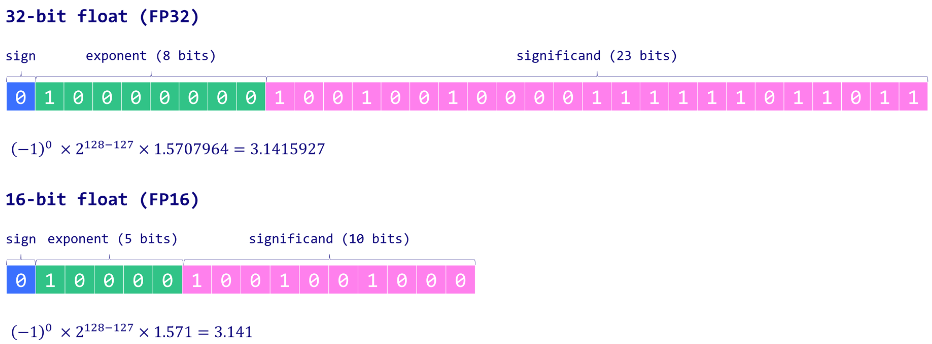
\includegraphics[width = 11cm]{./figure/float.png} \\ 
	{\footnotesize Source: \href{https://mlabonne.github.io/blog/posts/Introduction_to_Weight_Quantization.html}{Maxime Labonne}}
\end{figure}

\hspace{0.5cm}

You can represent every float like this:

$$(-1)^{\textcolor[RGB]{59,112,254}{S}}\cdot 2^{\textcolor[RGB]{49,195,135}{e}-bias} \cdot 1.\textcolor[RGB]{255,128,237}{m}$$
    
\end{vbframe}

% ------------------------------------------------------------------------------

\begin{vbframe}{Int8 Quantization (1)}

\textit{Since fp32 takes up too much memory, you can make use of int8 quantization to reduce the memory requirements}

\vfill

\begin{itemize}
    \item Real\_number = stored\_integer * scaling\_factor
    \item \textbf{Absmax quantization}: 
        \begin{itemize}
            \item $X_{quant} = \text{round}\left(\frac{127}{max{|\mathbf{X}|}} \cdot \mathbf{X}\right)$ 
        \end{itemize}
    \item \textbf{Zero-point quantization}: 
        \begin{itemize}
            \item $\text{scale} = \frac{255}{max(\mathbf{X}) - min(\mathbf{X})}$
            \item $\text{zeropoint} = -round(\text{scale}\cdot min(\mathbf{X})) - 128$
            \item $X_{quant} = round(\text{scale}\cdot \mathbf{X} + \text{zeropoint})$
        \end{itemize}
\end{itemize}

\vfill
    
\end{vbframe}

% ------------------------------------------------------------------------------

\begin{vbframe}{Int8 Quantization (2)}

\textit{We map a number from a fp32 to an int8 representation:}

\vfill

\begin{figure}
	\centering
	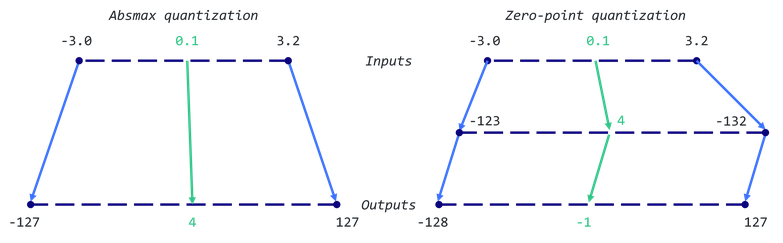
\includegraphics[width = 11cm]{./figure/intquant.png} \\ 
	{\footnotesize Source: \href{https://mlabonne.github.io/blog/posts/Introduction_to_Weight_Quantization.html}{Maxime Labonne}}
\end{figure}

\vfill

\textit{These quantizations reduce the amount of memory used by the model, also they further speed up computation by enabling integer computation instead of floating-point math!} 
    
\end{vbframe}

% ------------------------------------------------------------------------------

\begin{vbframe}{Model Parameters}

\vfill

Parameter size depends on chosen representation: \newline

\begin{itemize}
 	\item Pure fp32: $Mem_{model} = 4 ~bytes/param \cdot N_{params}$
 	\item fp16 or bf16: $Mem_{model} = 2 ~bytes/param \cdot N_{params}$
	\item int8: $Mem_{model} = 1 ~byte/param \cdot N_{params}$
\end{itemize}

\vskip8mm

It is practically common to use mixed representations: \newline

\begin{itemize}
 	\item fp32 + fp16
	\item fp32 + bf16
\end{itemize}

\vfill

\end{vbframe}

% ------------------------------------------------------------------------------

\begin{vbframe}{Optimizer States}

\vfill

AdamW: $Mem_{\text{AdamW}} = 8 ~bytes/param \cdot N_{params}$
\begin{itemize}
    % \item fp32 copy of parameters: 4 bytes/param
    \item Momentum: 4 bytes/param
	\item Variance: 4 bytes/param
\end{itemize}

\vskip3mm

bitsandbytes (8-bit optimizer): $Mem_{\text{optimizer}} = 2 ~bytes/param \cdot N_{params}$
\begin{itemize}
    % \item fp32 copy of parameters: 4 bytes/param
    \item Momentum: 1 byte/param
	\item Variance: 1 byte/param
\end{itemize}

\vskip3mm


% SGD-like optimizers with momentum: $Mem_{\text{optimizer}}= 8 \text{ bytes} /(\text{param}\cdot N_{params}$), 
% \begin{itemize}
% 	\item fp32 copy of parameters: 4 bytes/param
% 	\item Momentum: 4 bytes/param
% \end{itemize}

\vfill

\end{vbframe}

% ------------------------------------------------------------------------------

\begin{vbframe}{Gradients}

\vfill

They are usually stored in the same datatype as the model parameters. \newline

Their memory overhead contribution is: \newline

\begin{itemize}
 	\item fp32: $Mem_{grad} = 4 ~bytes/param \cdot N_{params}$
 	\item fp16 or bf16: $Mem_{grad} = 2 ~bytes/param \cdot N_{params}$
	\item int8: $Mem_{grad} = 1 ~byte/param \cdot N_{params}$
\end{itemize}

\vfill

\end{vbframe}

% ------------------------------------------------------------------------------

\begin{vbframe}{Activations}

\vfill

\begin{itemize}
 	\item GPUs are bottlenecked by memory, not FLOPs
 	\item Save GPU memory by recomputing activations of certain layers
	\item Various schemes for selecting which layers to clear
	\item They take some extra memory, but save even more
\end{itemize}

\vskip5mm

Total memory when training \textbf{using} activations: \newline
$Mem_{training} = Mem_{params} + Mem_{opt} + Mem_{grad} + Mem_{activ}$

\vskip5mm

Total memory when training \textbf{without} activations: \newline
$Mem_{training} = Mem_{params} + Mem_{opt} + Mem_{grad}$

\vskip5mm

% In the latter case, $Mem_{params}$, $Mem_{opt}$ and $Mem_{grad}$ are significantly smaller than in the former.

\vfill

\end{vbframe}

% ------------------------------------------------------------------------------

\endlecture
\end{document}
